\section{Redes Neuronales}

\noindent Las redes neuronales artificiales, redes neuronales simplemente a partir de ahora, se basan en el funcionamiento básico de las neuronas biológicas. Este tipo de células recogen señales externas, las procesan y producen una respuesta en consecuencia. 

\noindent En el caso de una neurona artificial, dados los valores de entrada de una observación, $\lbrace x_i\rbrace_{i=1}^p$, la neurona tiene asociada a cada uno de ellos un peso, $\lbrace \omega_i\rbrace_{i=1}^p$, y opcionalmente un sesgo $b$. Además la neurona tiene una función de activación $g(x)$. 

\noindent Una vez recogidos los valores, se hace una suma ponderada de ellos $z=b+\sum_{i=1}^p \omega_i x_i$ y la neurona produce el valor $g(z)$.

\begin{center}
%%Hay que pedirle a Carlos que lo edite por que yo la verdad que no se 
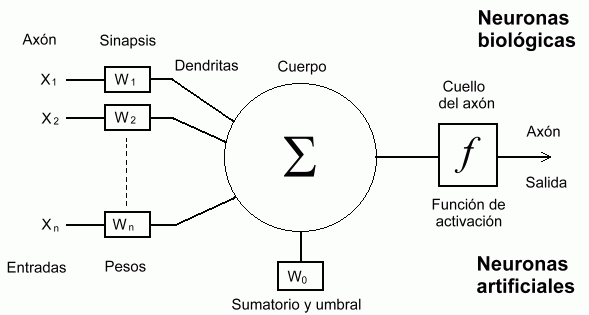
\includegraphics[scale=0.65]{Documentos Extra/neurona.png}
\end{center}

\noindent Una vez calculada la salida de la neurona, esta puede conectarse a otra, sirviendo los datos de salida de la primera neurona como datos de entrada de la siguiente. De manera  podemos tener capas de $m$ neuronas para producir $m$ salidas que sirvan como datos de entrada para la siguiente capa de neuronas.

\noindent Por último, puede haber capas al principio y al final para tareas como estandarizar, centrar los datos y deshacer dichas operaciones para producir una salida coherente. 
\newpage
\noindent La siguiente imagen es un esquema de una red neuronal con 7 capas de neuronas interconectadas donde la primera capa es de escalado y la última de desescalado. Se puede observar que se predicen las variables $y_1, y_2, y_3$ usando como entrada las variables $x_1,x_2,x_3,x_4$ 

\begin{figure}[h]
\centering
%%Hay que pedirle a Carlos que lo edite por que yo la verdad que no se 
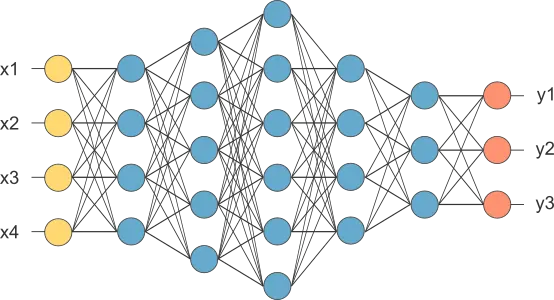
\includegraphics[scale=0.45]{Documentos Extra/red-neuronal-grande.png}
\caption{Imagen extraída directamente de www.neuraldesigner.com}
\end{figure}

\noindent Una vez detallado el proceso que se da dentro de una neurona hay que detallar los conceptos y elementos de la misma.

\begin{defi}
Se llama neurona a cada una de las transformaciones de los datos,  $g_m(\omega_m^T \textbf{x})$
\end{defi}
\begin{defi}
Al vector $\omega_m$ se le denomina \textit{vector de pesos} de la neurona, en particular, $\omega_{m0}$ se denomina \textit{sesgo} de la neurona. 
\end{defi}
\begin{defi}
Se define una capa de neuronas como un conjunto de ellas que producen un vector de salida, ya sea para servir como entrada de una capa posterior o como salida final. 
\end{defi}

\noindent Por tanto, utilizando las conexiones entre neuronas y entre sucesivas capas tenemos un algoritmo de regresión por búsqueda de proyecciones mediante la composición y combinación de distintas neuronas con pesos y funciones de activación distintas. 

\subsection{Proyection Pursuit Regression}

\noindent Sean un vector aleatorio \textbf{x} de longitud $p$, una variable objetivo $Y$ y una familia de vectores de parámetros de longitud $p$, $\lbrace \omega_m\rbrace_{m=1}^M$. Entonces el modelo de Regresión por Búsqueda de Proyecciones \textit{(PPR en inglés)} es de la forma :
\begin{equation}
f(\textbf{x})=\sum_{m=1}^M g_m(\omega_m^T \textbf{x})
\end{equation}

\noindent En este modelo las funciones $g_m$ no son especificadas y son estimaciones a lo largo de las direcciones de los vectores $\omega_m^T \textbf{x}$. Según Hastie, Tibshirani y Friedman \cite{Hastie 2001} para un $M$ lo suficiente grande y utilizando las $g_m$ apropiadas este modelo puede ayudar a la predicción de cualquier función continua real. 

%%Detallar

\noindent El uso de este modelo es complejo, debido a que hay una gran cantidad de parámetros de distintos tipos, obligando a utilizar distintos métodos de optimización. Asimismo, este tipo de modelos se utilizan solamente cuando se quiere predecir una variable, debido a su complejidad, que los hace difíciles de interpretar.

\noindent Sobre este modelo se sustentan las redes neuronales, que establecen previamente las funciones de activación $g_m$.

\noindent En el caso de las redes neuronales, el método de ajuste varía al modelo previamente descrito ya que las funciones están prefijadas 


\subsection{Red Neuronal de 2 capas }

\noindent En pos de la sencillez de los resultados, se detallará la  de una red neuronal de dos capas. El resto de casos $m\geq 2$, el proceso es análogo. Añadir que la situación es aquella en la que se quiere predecir $K$ variables objetivo a partir de observaciones de $p$ variables. 

\noindent La primera capa tiene los siguientes elementos:
\begin{itemize}
\item Como datos de entrada cada una de las observaciones $\textbf{x}$ de tamaño $p$ e incluimos en cada uno el término inicial $x_{0}=1$ de tal manera que hay $p+1$ datos de entrada.
\item Un total de $M$ unidades lo que provocará un conjunto $\lbrace z_m \rbrace$ de datos de salida.
\item Cada unidad de las $M$ tiene unos pesos $\alpha_m$ de dimensión $p+1$, donde la primera componente $\alpha_{m0}$ se denomina \textbf{sesgo}.
\item Una función de activación \textit{(Que puede o no ser lineal)} $g^{(1)}$.
\end{itemize}
\noindent De esta manera, tenemos que los datos de salida de esta primera capa son de la forma:
\begin{equation}
z_m=g^{(1)}(\alpha_m^T\textbf{x})
\end{equation}

\noindent De manera análoga tenemos una segunda capa de neuronas con los siguientes elementos:
\begin{itemize}
\item Como datos de entrada los $M$ resultados de la capa anterior, $z_m$ al que añadimos $z_0=1$ y denotaremos como el vector $\textbf{z}$ de longitud $M+1$.
\item Un total de $K$ unidades lo que provocará un conjunto $\lbrace t_k \rbrace$ de datos de salida.
\item Cada unidad de las $K$, tiene unos pesos $\beta_m$ de dimensión $M+1$ igual que en la anterior. 
\item Una función de activación \textit{(Que puede o no ser lineal)} $g^{(2)}$ que puede ser la misma que en la anterior o no.
\end{itemize}
\noindent De esta manera, tenemos que los datos de salida de esta primera capa son de la forma:
\begin{equation}
t_k=g^{(2)}(\beta_k^T\textbf{z})
\end{equation}
\noindent Hay que destacar que los datos deben estar escalados, o pueden serlo mediante una capa que los escale per sé.

\begin{defi}
Sea una matriz de datos $\textbf{X}$ de tamaño $n\times p$, resultado de observar las variables $X_1 \ldots X_p$, se llama \textit{capa de escalado} a la capa de neuronas con los siguientes elementos:
\begin{itemize}
\item Un vector de pesos con una sola componente igual a $1$ y el resto nulas. 
\item Una función de activación $g(z)=\frac{z-\mu_i}{\sigma_i}$ donde $\mu_i, \sigma_i$ son las media y desviación típica muestrales de cada variable.
\end{itemize}
\noindent El resultado de que la matriz de datos sea procesada por este tipo de capa es una matriz $\textbf{X}'$ centrada y estandarizada. 
\end{defi}

\subsection{Ajuste y uso de una Red Neuronal}

\noindent Una vez formulado el funcionamiento de una red neuronal, el ajuste de los pesos y sesgos de esta se puede plantear como un problema de minimización de la pérdida en función de los propios pesos, utilizando métodos de optimización numérica como el método del gradiente o el método de Quasi-Newton. 

\noindent Una vez ajustados los pesos el modelo resultante puede ser complejo de interpretar, pero proporciona predicciones que potencialmente pueden ser todo lo precisas que se requieran según \textit{[insertar el artículo de roberto]}. 

\noindent En este trabajo se han detallado los tipos más simples de redes neuronales y de neuronas, con las cuales ya se obtiene una gran capacidad de predicción. Sin embargo, hay estructuras neuronales como las redes convolucionales o las capas LSTM \textit{(Llamadas así por sus siglas en inglés Long-Short Term Memory)} que permiten modelizar sistemas en que los estados futuros son afectados por los estados anteriores como pudiera ser el precio de una acción bursátil o el tiempo atmosférico.